\chapter{Wprowadzenie}

W tym rozdziale omówię czym są grafy -- na początku przedstawię intuicyjne wyjaśnienie, po czym podam formalną definicję. Pojawią się także definicje pojęć związanych z grafami, które będą występować w kolejnych rozdziałach pracy. Następnie przytoczę przykłady znanych grafów, takich jak graf pełny czy graf cykliczny. W ostatniej sekcji przedstawię zastosowania grafów.

\section{Czym są grafy?}

\section{Definicje}

\subsection*{Graf ogólny, graf prosty}
\textbf{Graf} (\textbf{graf ogólny}, \textbf{multigraf}) $G$ jest parą $(V(G),E(G))$, gdzie $V(G)$ jest skończonym, niepustym zbiorem elementów zwanych \textbf{wierzchołkami}, a $E(G)$ jest skończoną rodziną nieuporządkowanych par elementów zbioru $V(G)$ zwanych \textbf{krawędziami} \footcite[20]{wilson} (tj. $E \subseteq \{\{u,v\} : u,v \in V(G)\}$). Zbiór $V(G)$ nazywamy zbiorem wierzchołków, a rodzinę $E(G)$ -- \textbf{rodziną krawędzi} grafu $G$; gdy nie ma możliwości pomyłki często są skracane do odpowiednio $V$ oraz $E$. (Niektóre definicje nie wymagają, aby zbiory $V$ oraz $E$ były skończone\footcite[143]{ross}, ale ponieważ w naszych zastosowaniach będziemy mieli do czynienia ze zbiorami skończonymi, przyjmiemy, że zbiory te są skończone).  Wierzchołki $u,v \in V$ są \textbf{połączone} krawędzią $\{u,v\}$ (lub krócej $uv$), gdy $\{u,v\} \in E$. 

\tikzset{every node/.style={fill,circle,scale=0.5,font=\huge}}

\begin{figure}
\centering
\begin{minipage}{.45\textwidth}
  \centering
  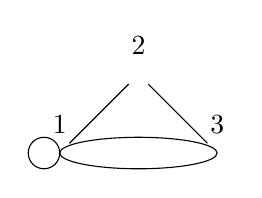
\begin{tikzpicture}
\filldraw 
(0,0) node[label=1](1){}
(1,1) node[label=2](2){} 
(2,0) node[label=3](3){};
\draw (0,0) arc (0:360:2mm);
\draw (2,0) arc (0:180:1 and 0.2);
\draw (0,0) arc (180:360:1 and 0.2);
\path[draw] (1)--(2);
\path[draw] (2)--(3);
\end{tikzpicture}
\captionsetup{justification=centering}
\caption{Przykład grafu~ogólnego} \label{fig:simple-graph}
\end{minipage}
\begin{minipage}{.45\textwidth}
  \centering
  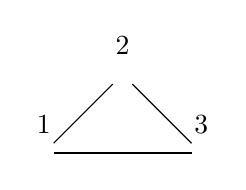
\begin{tikzpicture}
\filldraw 
(0,0) node[label=1](1){}
(1,1) node[label=2](2){} 
(2,0) node[label=3](3){};
\path[draw] (1)--(2);
\path[draw] (2)--(3);
\path[draw] (3)--(1);
\end{tikzpicture}
\captionsetup{justification=centering}
\caption{Przykład grafu~prostego} \label{fig:graph}
\end{minipage}
\end{figure}

Zauważmy, że taka definicja dopuszcza sytuację, w której dwa wierzchołki są połączone więcej niż jedną krawędzią (tzw. \textbf{krawędź wielokrotna}) oraz że wierzchołek jest połączony z samym sobą (tzw. \textbf{pętla}). Graf, który nie posiada krawędzi wielokrotnych oraz pętli nazywamy \textbf{grafem prostym}\footcite[19]{wilson}.

\subsection*{Sąsiedztwo}

Wierzchołki $u,v \in V$ są \textbf{sąsiednie} jeśli istnieje krawędź $uv$ (wierzchołki $u$ i $v$ są \textbf{incydentne} z tą krawędzią). Dwie krawędzie są \textbf{sąsiednie}, jeśli są incydentne z tym samym wierzchołkiem. 

\textbf{Stopień} wierzchołka $v \in V$ jest liczbą krawędzi incydentnych z $v$. \textbf{Wierzchołek izolowany} to wierzchołek stopnia 0, a \textbf{wierzchołek końcowy} -- stopnia 1.

Istnieją dwie standardowe reprezentacje grafów w pamięci komputera: jako \textbf{listy sąsiedztwa} lub jako \textbf{macierze sąsiedztwa}\footcite[29]{banachowski}. Pierwsza z nich polega na zapamiętaniu dla każdego wierzchołka listy wierzchołków z nim sąsiadujących. Druga zakłada, że wierzchołki są ponumerowane liczbami ze zbioru $\{1, 2,\ldots,n\}$ (gdzie $n$ oznacza moc zbioru $V$) i opiera się na stworzeniu macierzy wymiaru $n \times n$, której wyraz o indeksach $i,j$ jest równy liczbie krawędzi łączących wierzchołek o numerze $i$ z wierzchołkiem o numerze $j$.

Innym sposobem reprezentacji grafu za pomocą macierzy jest \textbf{macierz incydencji}. Jeśli krawędzie oznakujemy liczbami ze zbioru $\{1,2,\ldots,m\}$ (gdzie $m$ moc zbioru $E$), to jest to macierz o rozmiarze $n \times m$, której wyraz o indeksach $i,j$ jest równy 1, jeśli wierzchołek z numerem $i$ jest incydentny z krawędzią $j$, i równy 0 w przeciwnym przypadku.

\begin{figure}[H]
\centering
  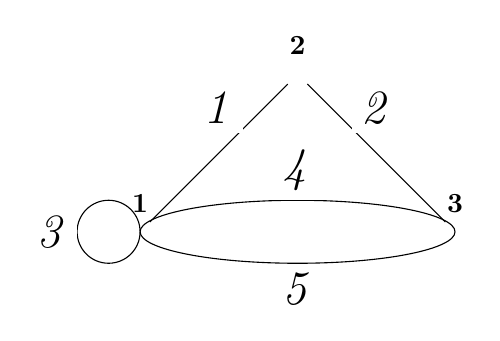
\begin{tikzpicture}
\filldraw 
(0,0) node[label=\textbf{1}](1){}
(2,2) node[label=\textbf{2}](2){} 
(4,0) node[label=\textbf{3}](3){};
\draw (0,0) arc (0:360:4mm) node [midway,left,fill=white] {\LARGE\textit{3}};
\draw (4,0) arc (0:180:2 and 0.4) node [midway,above,fill=white] {\LARGE\textit{4}};;
\draw (0,0) arc (180:360:2 and 0.4) node [midway,below,fill=white] {\LARGE\textit{5}};;
\path[draw] (1)--(2) node [midway,above=7pt,fill=white] {\LARGE\textit{1}};
\path[draw] (2)--(3) node [midway,above=7pt,fill=white] {\LARGE\textit{2}};
\end{tikzpicture}
\caption{}\label{fig:graph-edge-labeled}
\end{figure}

Macierz sąsiedztwa $A$ i macierz incydencji $M$ dla grafu z rysunku \ref{fig:graph-edge-labeled}:

\[A = 
 \begin{pmatrix}
  1 & 1 & 2 \\
  1 & 0 & 1 \\
  2 & 1 & 0 
 \end{pmatrix}, \hspace{20pt}
 M = 
 \begin{pmatrix}
  1 & 0 & 1 & 1 & 1 \\
  1 & 1 & 0 & 0 & 0 \\
  0 & 1 & 0 & 1 & 1 
 \end{pmatrix}
\]



\subsection*{Spójność}



\section{Przykłady grafów} \label{sec:common-graphs}
\section{Zastosowania grafów}